% !TeX spellcheck = en_US
\documentclass{beamer}

\mode<presentation> {
	\usetheme{Berkeley}
}

\usepackage{graphicx}
\usepackage{booktabs}
\usepackage[english]{babel}

\title[Sprint Review]{ROW5 Sprint 4 Review}

\author{ROW Team 5}
\institute[HvA]
{
	Amsterdam University of Applied Sciences \\
	\textit{https://rescueonwheels.github.io/}
}
\date{Januari 14, 2019}

\begin{document}

\begin{frame}
\titlepage
\end{frame}

\section{Introduction}
\begin{frame}{Introduction}
    \begin{center}
        \begin{tabular}{r|l}
             Christiaan van Arum & Developer \\
             \hline
             Rapha\"{e}l Bunck & Scrum Master \\
             \hline
             Nino van Galen & Developer \\
             \hline
             Martijn Vegter & Product Owner
         \end{tabular}
    \end{center}
\end{frame}

\begin{frame}
\frametitle{Overview}
\tableofcontents
\end{frame}

\section{Sensors and actuators}
\begin{frame}{Sensors and actuators}
	Sensor(s):
	\begin{itemize}
		\item Distance sensor (ultrasonic sensor HC-SR04)
	\end{itemize}
	
	Actuator(s):
	\begin{itemize}
		\item Custom double axis servo platform
	\end{itemize}
	
	Other:
	\begin{itemize}
		\item Fisheye lens
	\end{itemize}
\end{frame}

\section{Communication}
\begin{frame}{Communication}
	Rover $\leftrightarrow$ Cockpit:
	\begin{itemize}
		\item Socket.IO
	\end{itemize}

	Rover $\rightarrow$ Tincidunt:
	\begin{itemize}
		\item H.264 over HTTP
	\end{itemize}

	Cockpit $\leftarrow$ Controller:
	\begin{itemize}
		\item Bluetooth
		\item USB
	\end{itemize}
\end{frame}

\section{User Interface}
\begin{frame}{User Interface: Epicenter}
\begin{center}
	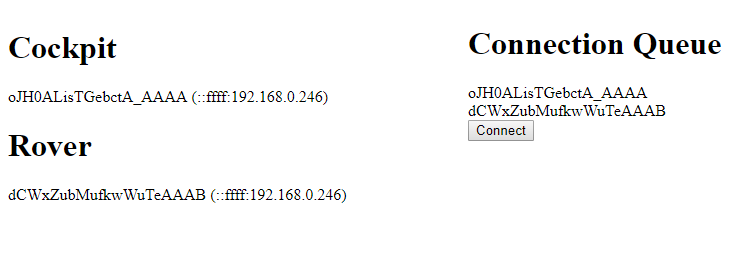
\includegraphics[width=\linewidth]{images/epicenter.png}
\end{center}
\end{frame}
\begin{frame}{User Interface: Chrome}
    \begin{center}
		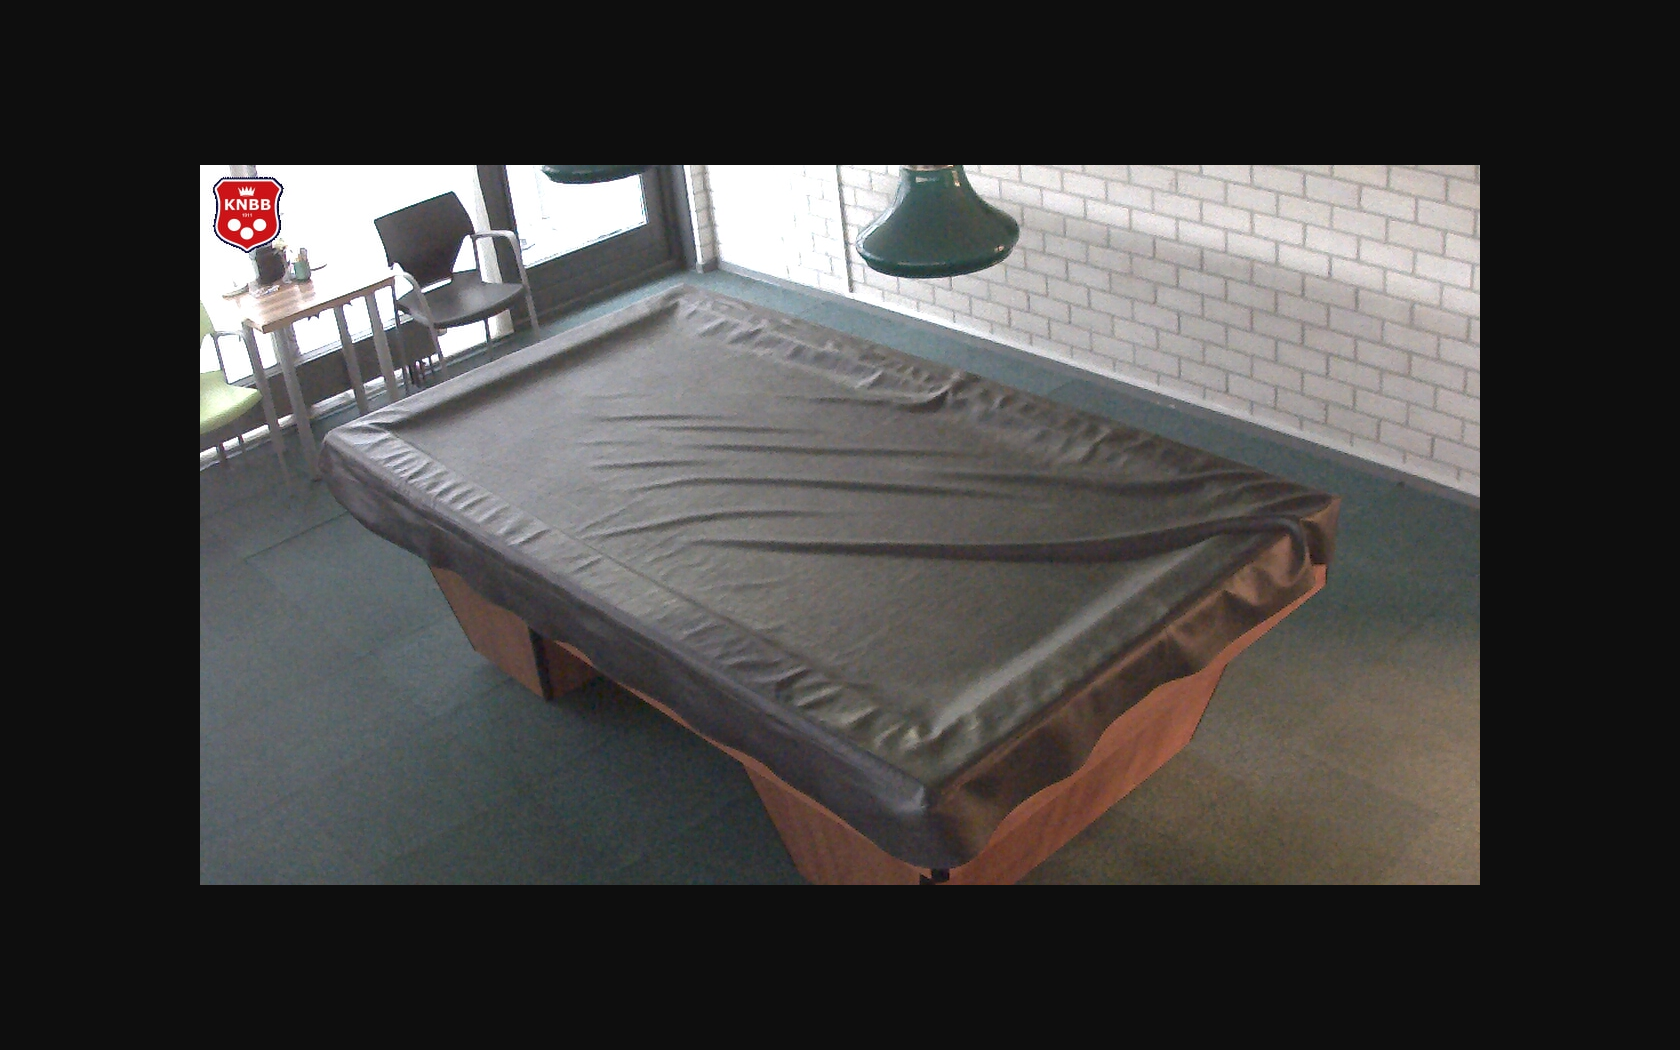
\includegraphics[width=\linewidth]{images/chrome.png}
	\end{center}
\end{frame}
\begin{frame}{User Interface: Tincidunt}
    \begin{center}
		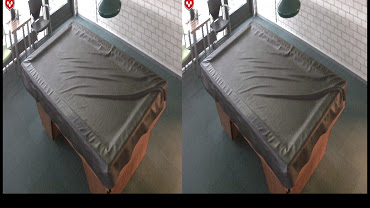
\includegraphics[width=\linewidth]{images/tincidunt.png}
	\end{center}
\end{frame}

\section{Operational scenario}
\begin{frame}{Operational scenario}
TODO
\end{frame}

\section{Documentation}
\begin{frame}{Documentation}
	\begin{itemize}
		\item Rover Rescue System - Business Case
		\item Rover Rescue System - (Technical) Documentation
		\item Rover Rescue System - Manual - Application
		\item Rover Rescue System - Manual - Epicenter
		\item Rover Rescue System - Manual - Rover
		\item Rover Rescue System - Project File
	 	\item Rover Rescue System - Sprint Review 1
	 	\item Rover Rescue System - Sprint Review 2
	 	\item Rover Rescue System - Sprint Review 3
	 	\item Rover Rescue System - Sprint Review 4
	\end{itemize}
\end{frame}

\section{Innovatation}
\begin{frame}{Innovatation}
	\begin{itemize}
		\item Virtual Reality as video output;
		\item Virtual Reality connected to the camera;
		\item Automated prevention systems:
		\begin{itemize}
			\item Auto-stop to prevent crashes;
			\item Auto-stop based on communication events;
			\item Auto-reset of camera view based on communication events;
			\item Scalable for large scale operations.
		\end{itemize}
	\end{itemize}
\end{frame}

\section{Scrum}
\begin{frame}{Scrum}
	\begin{itemize}
		\item Use of GitHub projects;
		\item Use of GitHub because of third-party integrations;		
		\item Use of ZenHub for automated issue tracking;
		\begin{itemize}
			\item Isssues
			\item Epics
			\item Pull Requests
		\end{itemize}
		\item Use of ZenHub for Burndown and Velocity tracking;
	\end{itemize}
\end{frame}
\begin{frame}{Scrum: Cumulative Flow}
	\begin{center}
		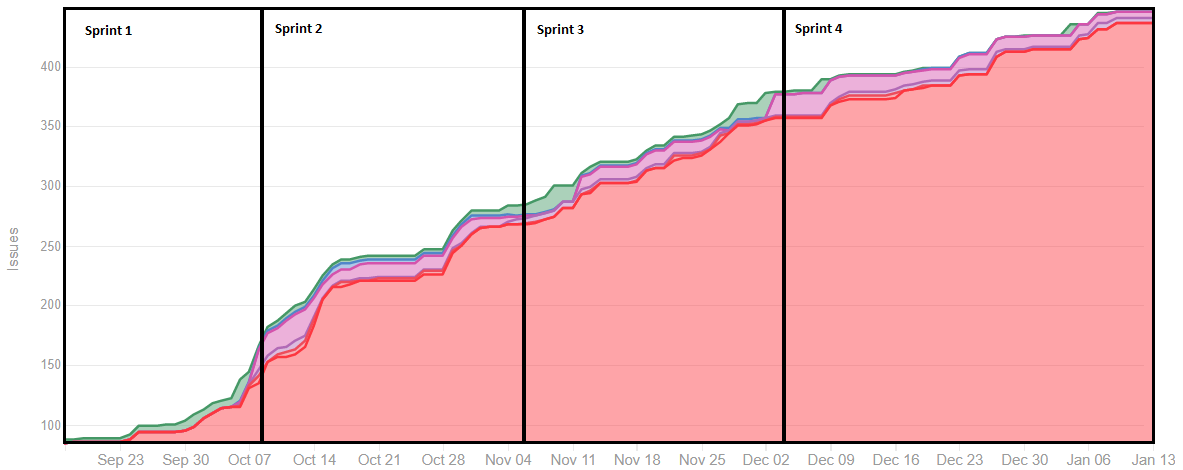
\includegraphics[width=\linewidth]{images/flow.png}
	\end{center}
\end{frame}
\begin{frame}{Scrum: Burndown sprint 1}
	\begin{center}
		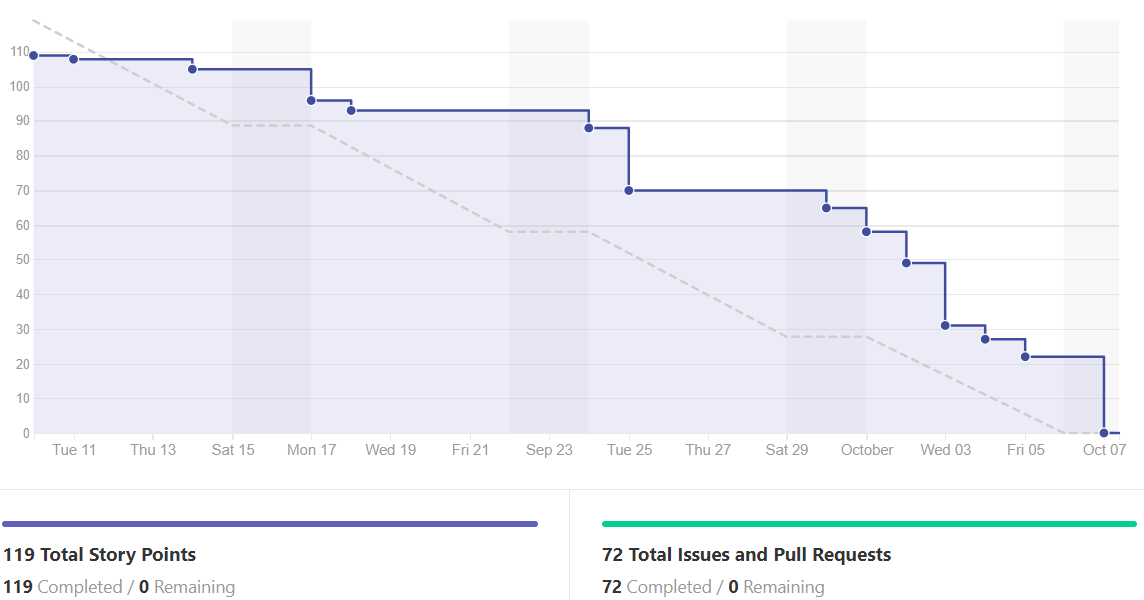
\includegraphics[width=\linewidth]{images/burn1.png}
	\end{center}
\end{frame}
\begin{frame}{Scrum: Burndown sprint 2}
	\begin{center}
		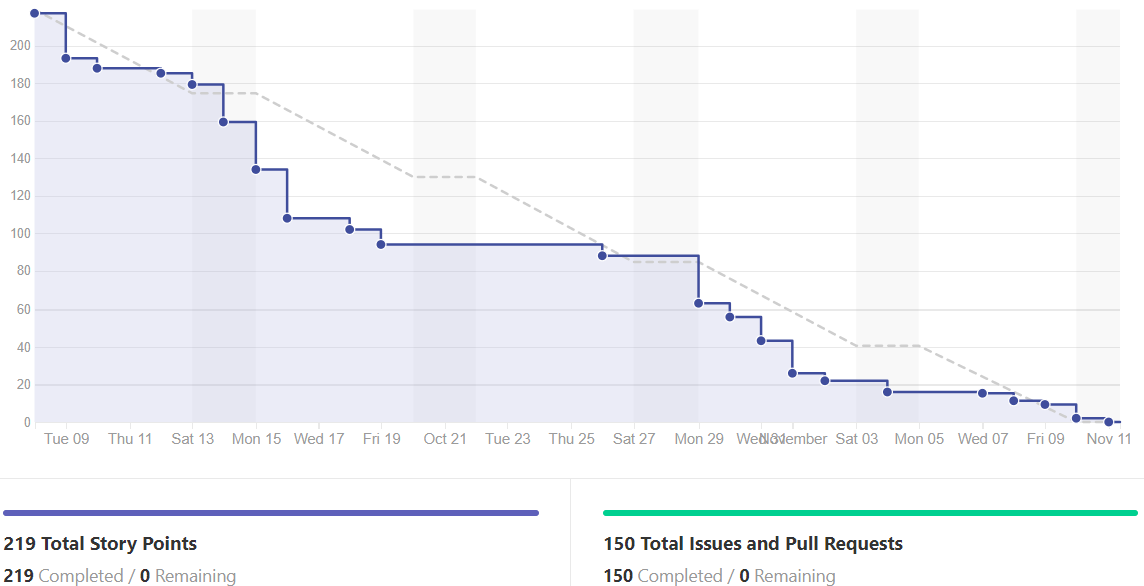
\includegraphics[width=\linewidth]{images/burn2.png}
	\end{center}
\end{frame}
\begin{frame}{Scrum: Burndown sprint 3}
	\begin{center}
		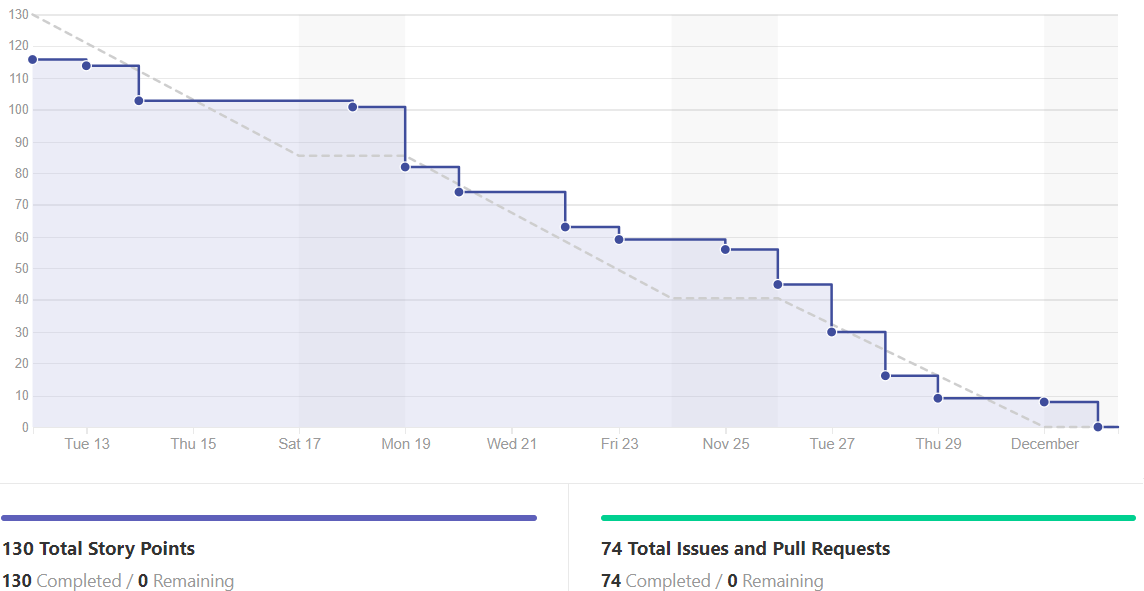
\includegraphics[width=\linewidth]{images/burn3.png}
	\end{center}
\end{frame}
\begin{frame}{Scrum: Burndown sprint 4}
	\begin{center}
		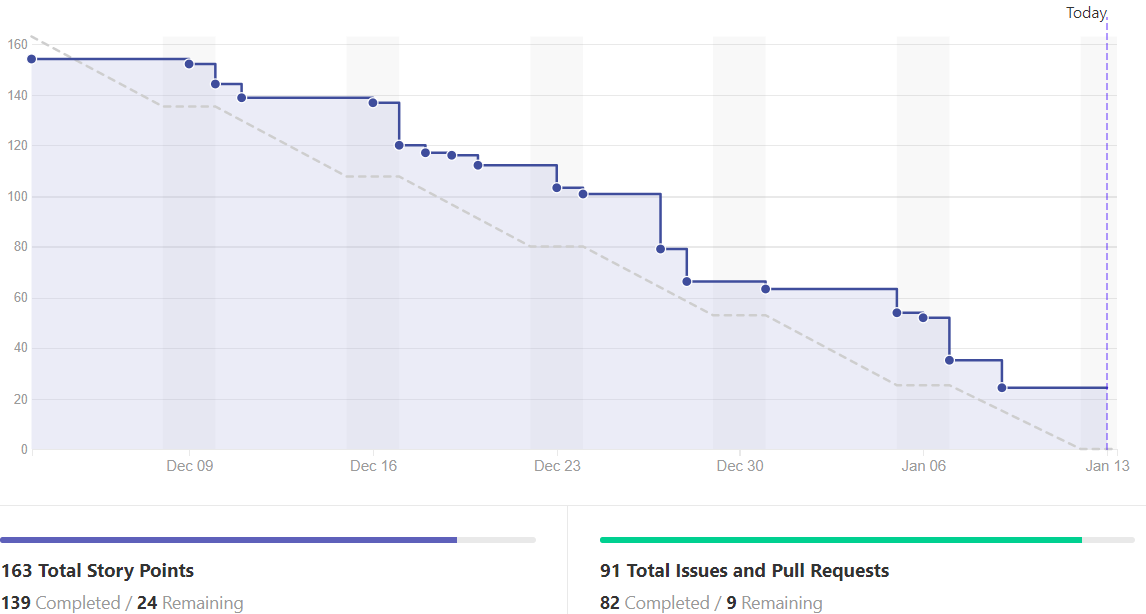
\includegraphics[width=\linewidth]{images/burn4.png}
	\end{center}
\end{frame}

\section{Quality assurance}
\begin{frame}{Quality assurance}
	\begin{itemize}
		\item Use of GIT submodules;
		\item Custom mocks for simulation usage;
		\item Protected branches with following rules:
			\begin{itemize}
				\item Require pull request reviews before merging;
				\item Require status checks to pass before merging
				\begin{itemize}
					\item Travis-CI used for tests and code style;
					\item CodeClimate used for unbiased code quality;
					\item Coveralls is used for code coverage.
				\end{itemize}
			\end{itemize}
		\item Definition of Done;
		\item Definition of Ready.
	\end{itemize}
\end{frame}

\section{End}
\begin{frame}
\Huge{\centerline{The End}}
\end{frame}

\end{document}